\section{子问题三：燃油替代支出预测}

\subsection{问题定义与难点}

任务三的目标是基于用户当前的出行习惯与车辆属性，预测其若继续驾驶燃油车每月需要承担的燃油支出 fuel\_expense\_per\_month。政策制定者可据此量化用户转型电动车的潜在节省金额。这是一个反事实推断问题，评分指标为 adj-$R^2$。

题面提示该任务``需理解车型+里程+地域对油价的复杂映射关系''。然而数据探索表明，燃油支出几乎由日通勤里程单变量决定（相关系数 0.952），并叠加一个标准差约 40 的加性噪声。

\subsection{探索性数据分析}

\subsubsection{日通勤与燃油支出的线性关系}

如图\ref{fig:t3_scatter}所示，燃油支出随日通勤里程线性增长。过原点 OLS 拟合得到系数 $\beta=8.395$，折外 adj-$R^2=0.905416$。

\begin{figure}[H]
\centering
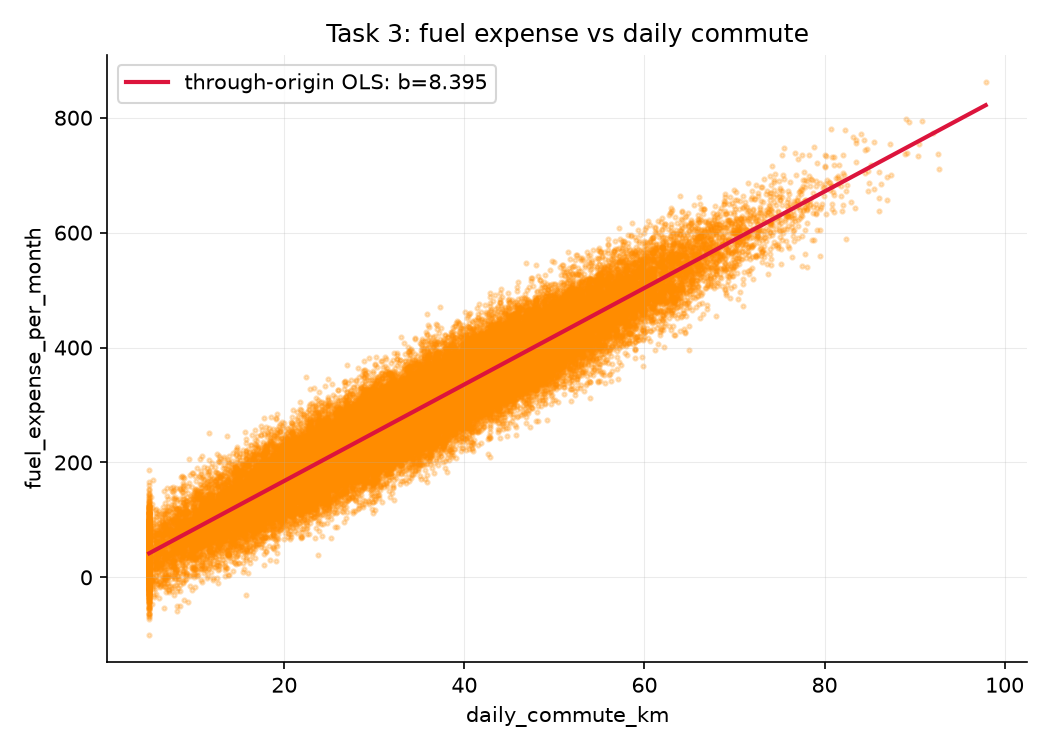
\includegraphics[width=0.8\textwidth]{figures/task3_fuel_scatter.png}
\caption{燃油支出与日通勤里程散点图及拟合线}
\label{fig:t3_scatter}
\end{figure}

\subsubsection{负值样本分布}

图\ref{fig:t3_dist}展示了燃油支出的分布，其中存在 271 个负值（最小值 $-99.7$），集中在低通勤区间。这些负值在业务语义上无效，但在统计上符合加性噪声的生成机制。

\begin{figure}[H]
\centering
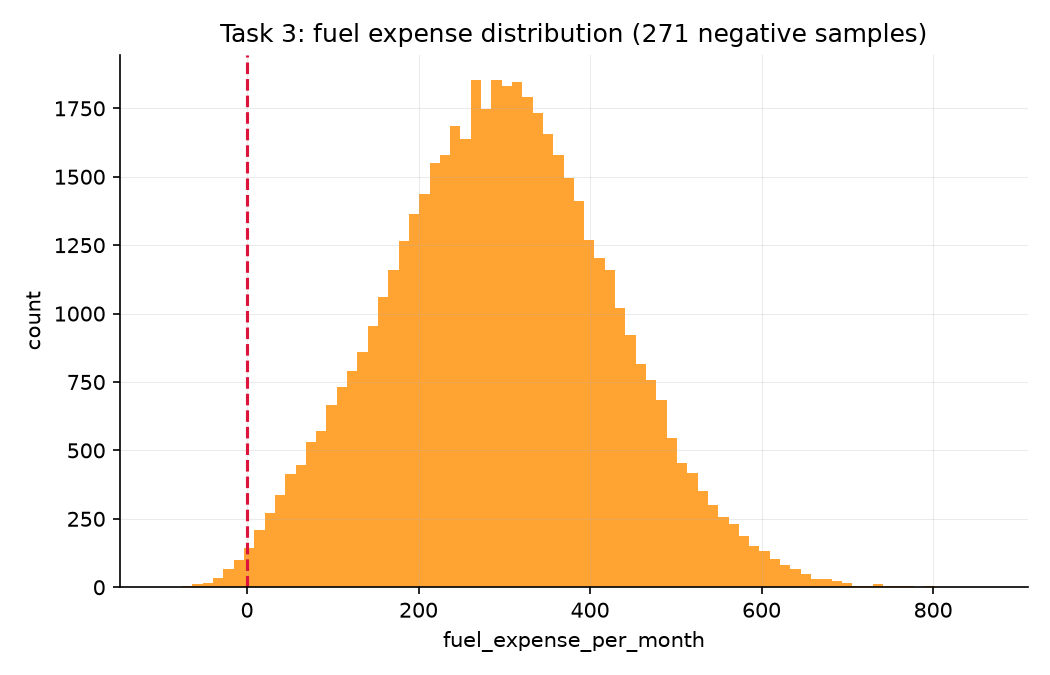
\includegraphics[width=0.8\textwidth]{figures/task3_target_dist.png}
\caption{燃油支出分布（含 271 个负值样本）}
\label{fig:t3_dist}
\end{figure}

\subsection{异常值处理策略}

针对负值样本，本文比较了四种处理策略：保留原值（过原点 OLS）、Huber 稳健回归、目标缩尾、删除负样本训练。结果如表\ref{tab:t3_outlier}所示。

\begin{table}[H]
\centering
\caption{任务三异常值处理策略对比（adj-$R^2$）}
\label{tab:t3_outlier}
\begin{tabular}{lcc}
\toprule
\textbf{策略} & \textbf{adj-$R^2$} & \textbf{说明} \\
\midrule
保留原值（过原点 OLS） & \textbf{0.905416} & 主方案 \\
Huber 稳健回归 & 0.905405 & 略降 \\
删除负样本训练 & 0.905369 & 略降 \\
目标缩尾（clip 到 $[0, Q_{99}]$） & 0.905280 & 明显下降 \\
\bottomrule
\end{tabular}
\end{table}

删除负值或对目标做缩尾、截断均使 adj-$R^2$ 下降，原因是负值样本与加性噪声结构一致，机械处理反而破坏了数据的真实分布。最终模型保留原始目标，不做对数变换与预测截断。

\subsection{特征块消融}

本文同样验证了题面建议的``车型+里程+地域''复杂映射是否有效。以日通勤为核心逐块加入特征，结果如表\ref{tab:t3_ablation}所示。

\begin{table}[H]
\centering
\caption{任务三特征块消融结果（adj-$R^2$）}
\label{tab:t3_ablation}
\begin{tabular}{lcc}
\toprule
\textbf{特征组合} & \textbf{特征数} & \textbf{adj-$R^2$} \\
\midrule
F0 核心（日通勤） & 1 & \textbf{0.905416} \\
F0 + 行程结构 & 4 & 0.905395 \\
F0 + 官方车型/地域交互 & 6 & 0.905374 \\
F0 + 车辆/地域 & 8 & 0.905379 \\
F0 + 其他信息 & 18 & 0.905371 \\
全特征 & 33 & 0.905311 \\
\bottomrule
\end{tabular}
\end{table}

与任务一一致，任何特征块的加入都无法提升 adj-$R^2$，官方提示的车型、地域交互在当前数据中不存在增益。

\subsection{残差诊断与非线性确认}

在日通勤过原点 OLS 的折内残差上训练浅层 LightGBM，其相对基线的 $\Delta R^2$ 为 $-0.000355$，Bootstrap 95\% 置信区间为 $[-0.000466, -0.000257]$，整体小于 0（表\ref{tab:t3_tree}）。树模型同样被淘汰。

\begin{table}[H]
\centering
\caption{任务三树模型残差确认}
\label{tab:t3_tree}
\begin{tabular}{lccc}
\toprule
\textbf{方案} & \textbf{$R^2$} & \textbf{$\Delta R^2$（Bootstrap 95\% CI）} & \textbf{结论} \\
\midrule
稀疏基线 & 0.905418 & -- & 主方案 \\
残差 LightGBM & 0.905056 & $[-0.000466, -0.000257]$ & 淘汰 \\
\bottomrule
\end{tabular}
\end{table}

\subsection{最终模型}

任务三的最终模型为：

\begin{equation}
\hat{y}_3 = \beta \cdot daily\_commute\_km, \quad \beta = 8.3947643
\label{eq:t3}
\end{equation}

在 5 折 $\times$ 3 种子最终确认中，adj-$R^2$ 均值为 0.905416 $\pm$ 0.000002。剩余约 40 的残差标准差接近不可约的加性噪声，说明在当前特征集合下模型已逼近预测上限。
